\documentclass[tikz,border=12pt]{standalone}
% Estilo comum dos esquemas vetoriais das aulas da GA033.
\usepackage[T1]{fontenc}
\usepackage[utf8]{inputenc}
\usepackage{lmodern}
\usepackage{amsmath,amssymb}
\usetikzlibrary{arrows.meta,positioning,calc,fit,matrix,decorations.pathreplacing,backgrounds,shapes.geometric}
\definecolor{lnccblue}{HTML}{075AC0}
\definecolor{ink}{HTML}{242A31}
\definecolor{muted}{HTML}{647080}
\definecolor{lightblue}{HTML}{EFF5FC}
\definecolor{teal}{HTML}{197C83}
\definecolor{orange}{HTML}{BC6A16}
\tikzset{
  every node/.style={font=\sffamily\fontsize{15}{18}\selectfont,text=ink},
  box/.style={draw=lnccblue,line width=0.9pt,fill=lightblue,inner sep=9pt,align=center},
  flow/.style={-{Stealth[length=3mm,width=2mm]},draw=lnccblue,line width=1pt},
  point/.style={circle,draw=lnccblue,fill=white,line width=1.2pt,minimum size=3.2mm,inner sep=0pt},
  label/.style={font=\sffamily\fontsize{13}{16}\selectfont,text=muted},
  heading/.style={font=\sffamily\bfseries\fontsize{16}{19}\selectfont,text=lnccblue}
}
% Impede setas horizontais involuntariamente invertidas após editar os nós.
\newdimen\origemseta
\newdimen\destinoseta
\newcommand{\verificarsetadireita}[2]{%
  \pgfextractx{\origemseta}{\pgfpointanchor{#1}{east}}%
  \pgfextractx{\destinoseta}{\pgfpointanchor{#2}{west}}%
  \advance\origemseta by 4mm%
  \ifdim\destinoseta>\origemseta\else
    \PackageError{diagramas}{Conector sem espaco entre #1 e #2}{Afaste os nos antes de compilar.}%
  \fi
}

\begin{document}
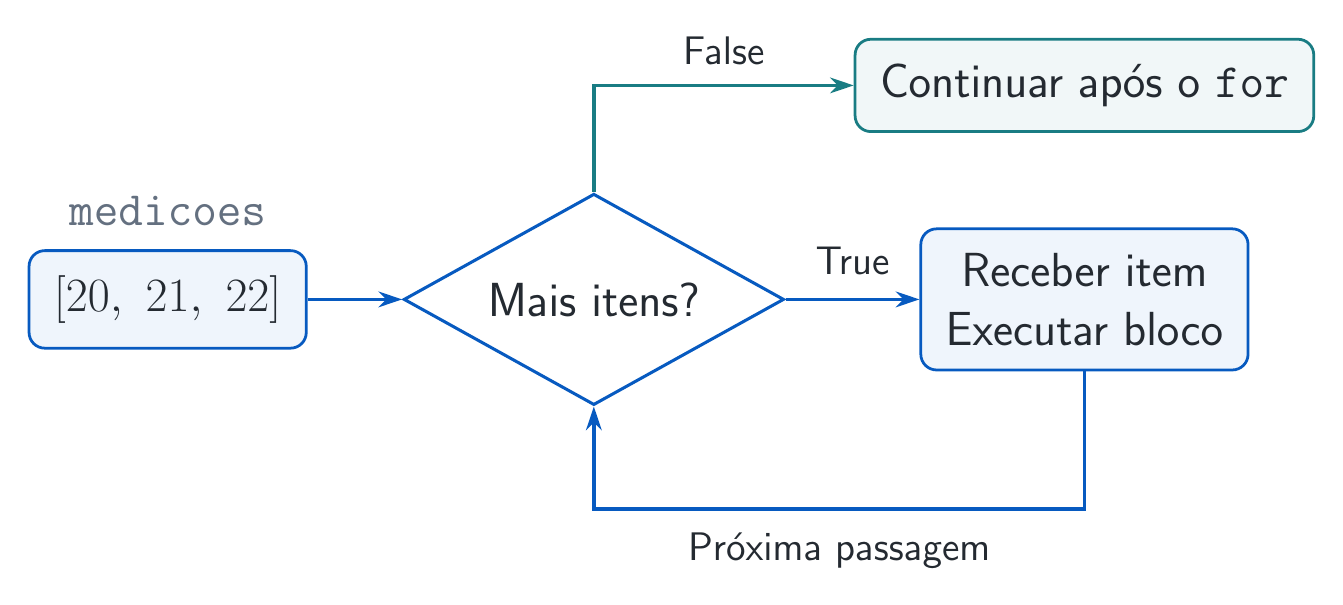
\begin{tikzpicture}[
  every node/.append style={font=\sffamily\fontsize{17}{21}\selectfont},
  etapa/.style={draw=lnccblue,fill=lightblue,rounded corners=2mm,
    line width=1pt,align=center,inner sep=9pt,minimum height=.9cm},
  seta/.style={-{Stealth[length=3mm,width=2mm]},draw=lnccblue,line width=1.2pt}
]
\node[etapa] (dados) {$[20,\ 21,\ 22]$};
\node[above=5pt,text=muted] at (dados.north) {\texttt{medicoes}};
\node[diamond,aspect=1.8,draw=lnccblue,fill=white,line width=1.1pt,
  inner sep=7pt,right=12mm of dados] (teste) {Mais itens?};
\node[etapa,right=17mm of teste] (bloco) {Receber item\\Executar bloco};
\node[etapa,draw=teal,fill=teal!6,above=12mm of bloco]
  (fim) {Continuar após o \texttt{for}};
\coordinate (retorno) at ($(teste.south)+(0,-13mm)$);
\verificarsetadireita{dados}{teste}
\verificarsetadireita{teste}{bloco}
\draw[seta] (dados.east) -- (teste.west);
\draw[seta] (teste.east) -- (bloco.west)
  node[midway,above=5pt,font=\sffamily\fontsize{15}{18}\selectfont] {True};
\draw[seta,draw=teal] (teste.north) |- (fim.west);
\node[above=4pt,font=\sffamily\fontsize{15}{18}\selectfont]
  at ($(teste.north |- fim.west)!0.5!(fim.west)$) {False};
\draw[seta] (bloco.south) |- (retorno) -- (teste.south);
\node[below=5pt,font=\sffamily\fontsize{15}{18}\selectfont]
  at ($(retorno)!0.5!(retorno -| bloco.south)$) {Próxima passagem};
\end{tikzpicture}
\end{document}
